\section{Entanglement and its applications}

A n-qubit state $\statepsi$ $(n \geq 2)$ is called \underline{entangled} if it cannnot be written 
as a tensor product of single-qubit states; i.e

\begin{equation}
    \statepsi \neq \ket{\psi_{n-1}} \otimes \cdots \otimes \ket{\psi_0}
\end{equation}

Example: Bell states, also denoted EPR states (Einstein, Podolsky, Rosen):

\begin{align*}
    \ket{\beta_{00}} &= \frac{1}{\sqrt{2}} (\ket{00} + \ket{11}) \\
    \ket{\beta_{01}} &= \frac{1}{\sqrt{2}} (\ket{01} + \ket{10}) \\
    \ket{\beta_{10}} &= \frac{1}{\sqrt{2}} (\ket{00} - \ket{11}) \\
    \ket{\beta_{11}} &= \frac{1}{\sqrt{2}} (\ket{01} - \ket{10}) \\
\end{align*}

\begin{figure}[H]
    \centering
    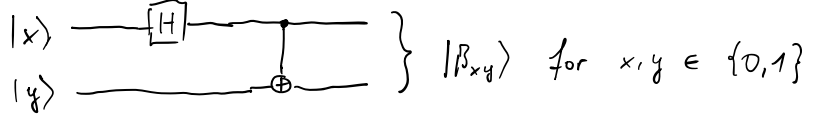
\includegraphics[scale=0.5]{chapters/res/circuit-bell-states.png}
    \caption{Quantum circuit to create Bell states}
\end{figure}


\subsection{Quantum teleportation}

Scenario: two (experimental physicists) Alice and Bob, are far away from each other

\begin{figure}[H]
    \centering
    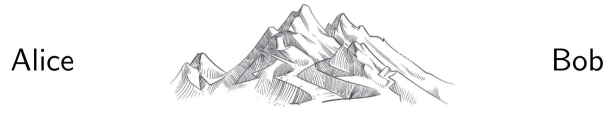
\includegraphics[scale=0.5]{chapters/res/alice-bob-mountains.png}
\end{figure}

When visiting each other a long time ago, they generated the EPR pair $\ket{\beta_{00}}$ each keeping on qubit of the pair.
Alice's task is to send another (unkown) qubit $\statepsi$ to Bob.
Note: Measurement is not an option.

\begin{figure}[H]
    \centering
    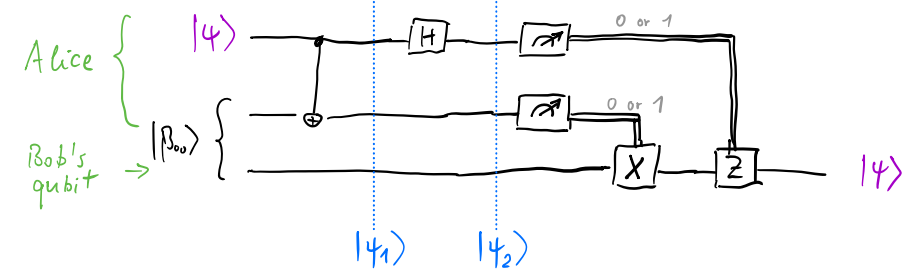
\includegraphics[scale=0.42]{chapters/res/circuit-teleporting-psi.png}
    \caption{Quantum circuit for teleporting $\statepsi$}
\end{figure}

Input:

\begin{equation*}
    \statepsi \ket{\beta_{00}} = (\alpha \ket{0} + \beta \ket{1}) \otimes \ket{\beta_{00}} 
        = \frac{1}{\sqrt{2}} \left[\alpha \ket{0} (\ket{00} + \ket{11}) + \beta \underbrace{\ket{1} (\ket{00} + \ket{11}}_{\text{CNOT}})\right]
\end{equation*}

after CNOT:
\begin{equation*}
    \ket{\psi_1} = \frac{1}{\sqrt{2}} 
        \left[\alpha \ket{0} (\ket{00} + \ket{11}) + \beta \ket{1} (\ket{{\color{red}1}0} + \ket{{\color{red}0}1})\right]
\end{equation*}

after Hadamard:
\begin{align*}
    \ket{\psi_2} &= \frac{1}{2} 
        [\alpha (\ket{0} + \ket{1})  \cdot
            (\ket{00} + \ket{11})]
        + \beta (\ket{0} - \ket{1}) \cdot 
            ((\ket{10} + \ket{01})) \\
    %
    &= \frac{1}{2} (\alpha \ket{000} + \alpha \ket{011} \alpha \ket{100} + \alpha \ket{111})
        + \beta \ket{010} + \beta \ket{001} - \beta \ket{110} - \beta \ket{101}) \\
    %
    &= \frac{1}{2} (\alpha \ket{000} + \alpha \ket{011} + \alpha \ket{100} + \alpha \ket{111}) + 
        \beta \ket{010} + \beta \ket{001} - \beta \ket{110} - \beta \ket{101} \\
    %
    &= \frac{1}{2} (\ket{00} (\alpha \ket{0} + \beta \ket{1}) + \ket{01} (\alpha \ket{1} + \beta \ket{0}))
        + \ket{10} (\alpha \ket{0} - \beta \ket{1}) + \ket{11} (\alpha \ket{1} - \beta \ket{0}))
\end{align*}

Now Alice measures her qubits w.r.t computational basis, e.g. projective measurement with 

\begin{align*}
    P_1 &= \ket{00} \bra{00} \otimes I, \quad P_2 = \ket{01} \bra{10} \otimes I \\ 
    P_3 &= \ket{10} \bra{10} \otimes I, \quad P_2 = \ket{11} \bra{11} \otimes I \\ 
\end{align*}

If Alice measures $\ket{00}$, then $\ket{\psi_2}$ will collapse to 
\begin{equation*}
    \ket{00} (\alpha \ket{0} + \beta \ket{1}) = \ket{00} \underbrace{\statepsi}_{\text{Qubit at Bob's place}}
\end{equation*}

similarly:

\begin{align*}
    00 &\mapsto \alpha \ket{0} + \beta \ket{1} \\
    01 &\mapsto \alpha \ket{1} + \beta \ket{0} \\
    10 &\mapsto \alpha \ket{0} - \beta \ket{1} \\
    11 &\mapsto \alpha \ket{1} - \beta \ket{0} 
\end{align*}

Alice transmits her measurement result to Bob (classical information), Bob then applies
Pauli-X and / or Pauli-Z to recover $\statepsi$. Even though wavefunction collapse is 
instantaneous, no faster-than-light transfer possible due to required classical communication.

\subsection{EPR and the Bell inequality}
EPR: Einstein, Podolsky, Rosen
EPR paper: \textit{"Can quantum mechanical description of physical relatiy be considered complete?"} (1935) \\
%
The another argue that quantum mechanics is incomplete since it lacks certain "elements of reality" 
(property can be predicted with certainity).

Scenario: Alice and Bob are far from each other, but share the entangled two-qubit "spin-singlet" state
\begin{equation*}
    \ket{\beta_{11}} = \frac{1}{\sqrt{2}} (\ket{01} - \ket{10})
\end{equation*}

Alice and Bob measure the observable $\vec{v} \circ  \vec{\sigma} = v_1 X + v_2 Y + v_3 Z$ 
(with $v \in \mathbb{R}^3, \norm{\vec{v}} = 1$) on their respective qubit.
(Recall $\vec{v} \circ \vec{\sigma}$ is Hermitian and unitary, and has eigenvalues $\pm 1$)

Alice performs her measurement immediately before Bob.
Example:
\begin{itemize}
    \item $\vec{v} = (0, 0, 1)^T$, observable $Z = 1 \cdot \ket{0} \bra{0} + (-1) \cdot \ket{1} \bra{1}$
        (standard measurement) \\
        if alice measures eigenvalue
        \begin{align*}
            1: &\quad \text{wavefunction collapses to } \ket{01} \\
            0: &\quad \text{wavefunction collapses to } \ket{10}
        \end{align*}
        $\leadsto$ Bob will always obtain the opposite measurement result.
\end{itemize}